\section{1174054 - Aulyardha Anindita}

\subsection{Teori}
\begin{enumerate}
\item Binary Classification \\
Binary Classification adalah suatu tugas mengklafisikan himpunan yang didalamnya terdapat elemen-elemen yang dimasukkan ke dalam kelompok berdasarkan aturan klasifikasi. Beberapa katakteristik tersebut contohnya tes medis digunakan untuk mengetahui suatu pasien memiliki penyakit tertentu atau tidak. dan properti klasifikasi tersebut adalah keberadaan penyakit dari pasien.\\

Binary Classification digunakan untuk tujuan praktis dalam banyak masalah klasifikasi biner, dan kedua kelompok tersebut tidak simetris daripada akurasi secara keseluruhan, proporsi relatif dari berbagai macam kesalahan yang menarik. Contohnya, dalam pengujian medis tadi, false positif maksudnya mendeteksi penyakit ketika ada sedangkan untuk false negatif artinya tidak mendeteksi penyakit ketika ada.\\

Ada banyak metrik yang bisa digunakan dalam mengukur kinerja klasifikasi dan prediksi. misalnya dapat dilihat pada gambar berikut:
\begin{figure}[H]
		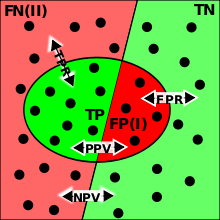
\includegraphics[width=4cm]{figures/1174054/2/binary.png}
		\centering
		\caption{Binary Classification}
\end{figure}

Bagian kiri dan kanan masing-masing memiliki instance yang sebenarnya ada dan tidak memiliki konndisi. Sedangkan bentuk oval tersebut berisi instance yang diklasifikasikan atau diprediksi sebagai positif atau negatif.

\item Supervised Learning, Unsupervised Learning, dan Clustering
\begin{itemize}
\item Supervised Learning \\
Dalam Supervised Learning, suatu program komputer diberikan dataset pelatihan yang kemudian diberi label dengan nilai output yang sesuai, dan fungsi tersebut akan ditentukan berdasarkan pada dataset. Fungdi atau algoritma tersebut kemudian akan digunakan untuk mengklasifikasian data abru untuk memprediksi nilai-nilai output yang sesuai dengan asumsi bahwa data baru sesuai dengan aturan dan fungsi yang digunakan. Berikut adalah contoh supervised learning:
\begin{figure}[H]
		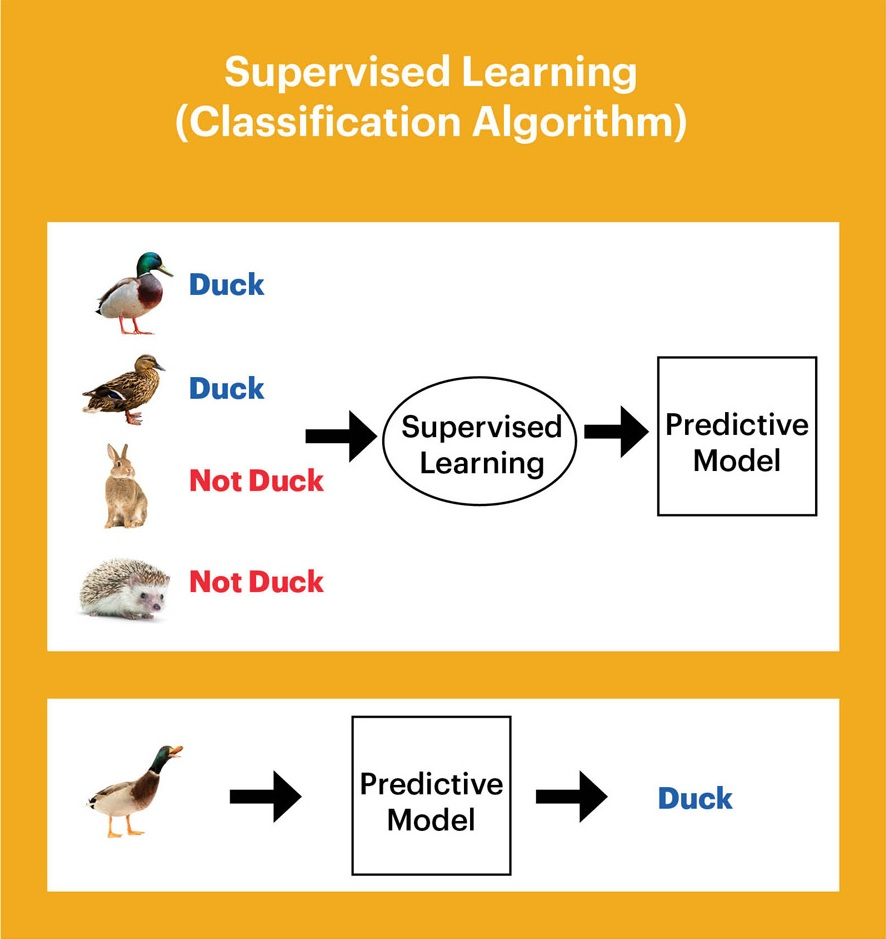
\includegraphics[width=4cm]{figures/1174054/2/supervised.jpg}
		\centering
		\caption{Supervised Learning}
\end{figure}

\item Unsupervised Learning \\
Dalam Unsupervised Learning, dataset pelatihan tidak memiliki label nilai output yang sesuai, karena tidak ada jawaban benar untuk dipelajari, tujuan algoritma ini adalah untuk mengungkap pola-pola menarik yang dapat ditemukan dalam data, dan data baru akan membantu untuk mengonfirmasi atau membatalkan pola-pola yang ditemukannya. Berikut adalah contoh Unsupervised Learning:
\begin{figure}[H]
		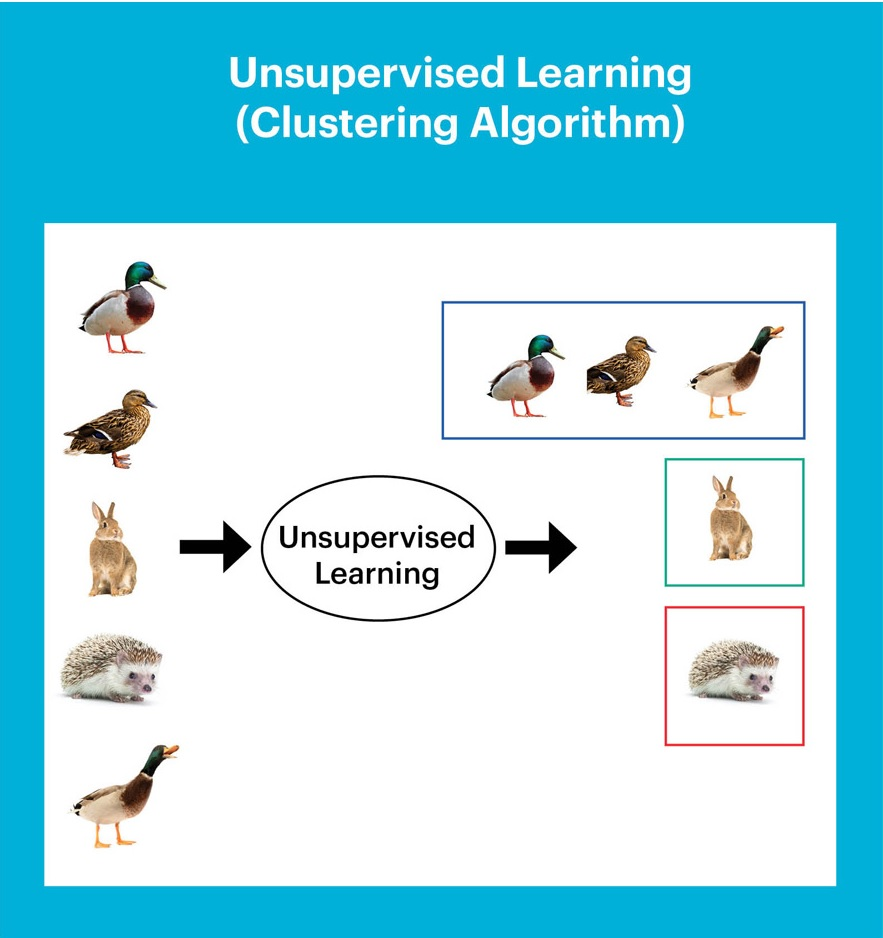
\includegraphics[width=4cm]{figures/1174054/2/unsupervised.jpg}
		\centering
		\caption{Unsupervised Learning}
\end{figure}

\item Clustering \\
Clustering adalah suatu teknik yang masuk kedalam kelompok Unsupervised Learning yang  merupakan teknik dimana mesin akan bekerja atau belajar sendiri tanpa diajari bagaimna cara memecahkan masalahnya. Contohnya, Kita memiliki sebuah data, yaitu data pelanggan yang berisi jenis kelamin, besarnya penghasilan dan besarnya pembelian produk. Maka dengan algoritma Clustering kita dapat mengetahui pelanggan kita akan dikelompokkan kedalam beberapa kluster dengan sendirinya.Misalnya ada pelanggan yang pelit, pelanggan yang royal dan lain sebagainya. Contohnya, Bisa kita lihat bagaimana sebuah teknik clustering bisa mengelompokkan data ke dalam beberapa kluster.
\begin{figure}[H]
		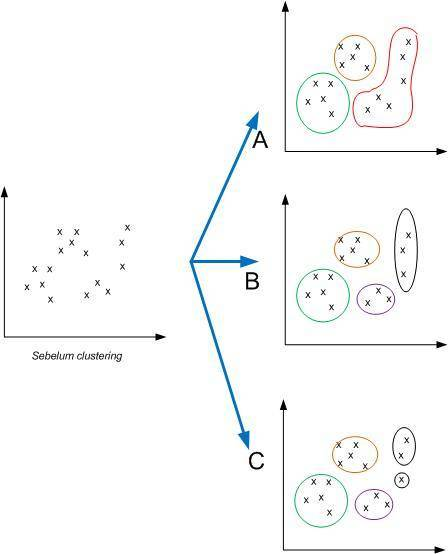
\includegraphics[width=4cm]{figures/1174054/2/clustering.jpg}
		\centering
		\caption{Clustering}
\end{figure}
\end{itemize}

\item Evaluasi dan Akurasi \\
Evaluasi merupakan suatu cara atau teknik dalam mengevaluasi seberapa baik model bekerja dengan mengukur akurasinya. Sedangkan akurasi adalah suatu persentase kasus yang diklasifikasikan dengan benar. Kita bisa menganalisis suatu kesalahan yang dibuat dengan model atau tingkat confusion dengan menggunakan matriks confusion. Berikut adalah contoh klasifikasi biner yang menunjukkan berapa kali model telah membuat prediksi yang benar dari objek.
\begin{figure}[H]
		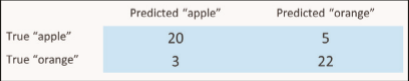
\includegraphics[width=4cm]{figures/1174054/2/evaluasi.png}
		\centering
		\caption{Evaluasi}
\end{figure}
Dalam tabel diatas,baris True Apple dan True Orange mengacu pada suatu kasus dimana objek itu sebenarnya sebuah apel atau sebenarnya jeruk. Kolom merujuk pada prediksi yang dibuat oleh model. Kita melihat bahwa ada 20 apel yang diprediksi dengan benar, sementara ada 5 apel yang dalah diidentifikasi sebagai jeruk. Sehingga, matriks confusion harus memiliki semua nol, kecuali untuk diagonal sehingga kita dapat menghitung akurasi dengan menambahkan angka secara diagonal seperti pada gambar berikut :
\begin{figure}[H]
		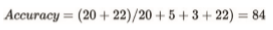
\includegraphics[width=4cm]{figures/1174054/2/akurasi.png}
		\centering
		\caption{Akurasi}
\end{figure}

\item Cara Membuat dan Membaca Confusion Matrix \\
Confusion Matrix adalah suatu matrix yang memberikan informasi perbandingan hasil klasifikasi yang dilakukan pada sistem atau model dengan hasil klasifikasi sebenarnya. Confusion Matrix berbentuk tabel matriks yang menggambarkan suatu kinerja model klasifikasi dari serangkaian data uji yang nilai sebenarnya diketahui. \\
Berikut cara membuat dan membaca confusion matrix : pertama, tentukan terlebih dahulu pokok permasalahan dan atributnya. kedua, buatlah pohon keputusan dan data testingnya. ketiga, carilah nilai a,b,c dan d. Selanjutnya, cari nilai recall, precesion, accuracy serta seeror rate. Berikut contoh Confusion Matrix :
\begin{figure}[H]
		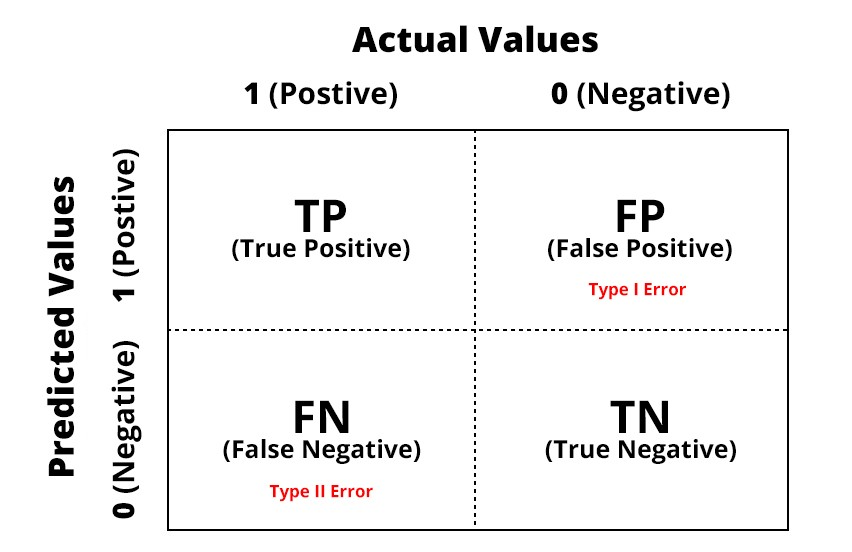
\includegraphics[width=4cm]{figures/1174054/2/confusion.jpeg}
		\centering
		\caption{Confusion Matrix}
\end{figure}

\item Cara Kerja K-fold Cross Validation 
\begin{itemize}
\item Pertama, total instance bagi menjadi N bagian
\item Fold pertama merupakan bagian peertama yang menjadi data uji atau testing data dan sisanya menjadi training data
\item Kemudian, hitung akurasi dari porsi data dengan menggunakan persamaan
\item Fol kedua, adalah bagian kedua dengan menjadi data uji atau testing data dan sisanya merupakan training data
\item Lalu, hitung akurasi dari porsi data tersebut
\item Lakukan hal tersebut, sampai habis mencapai fold ke-K
\item Setelah itu, hitung rata-rata akurasi K
\end{itemize}
\begin{figure}[H]
		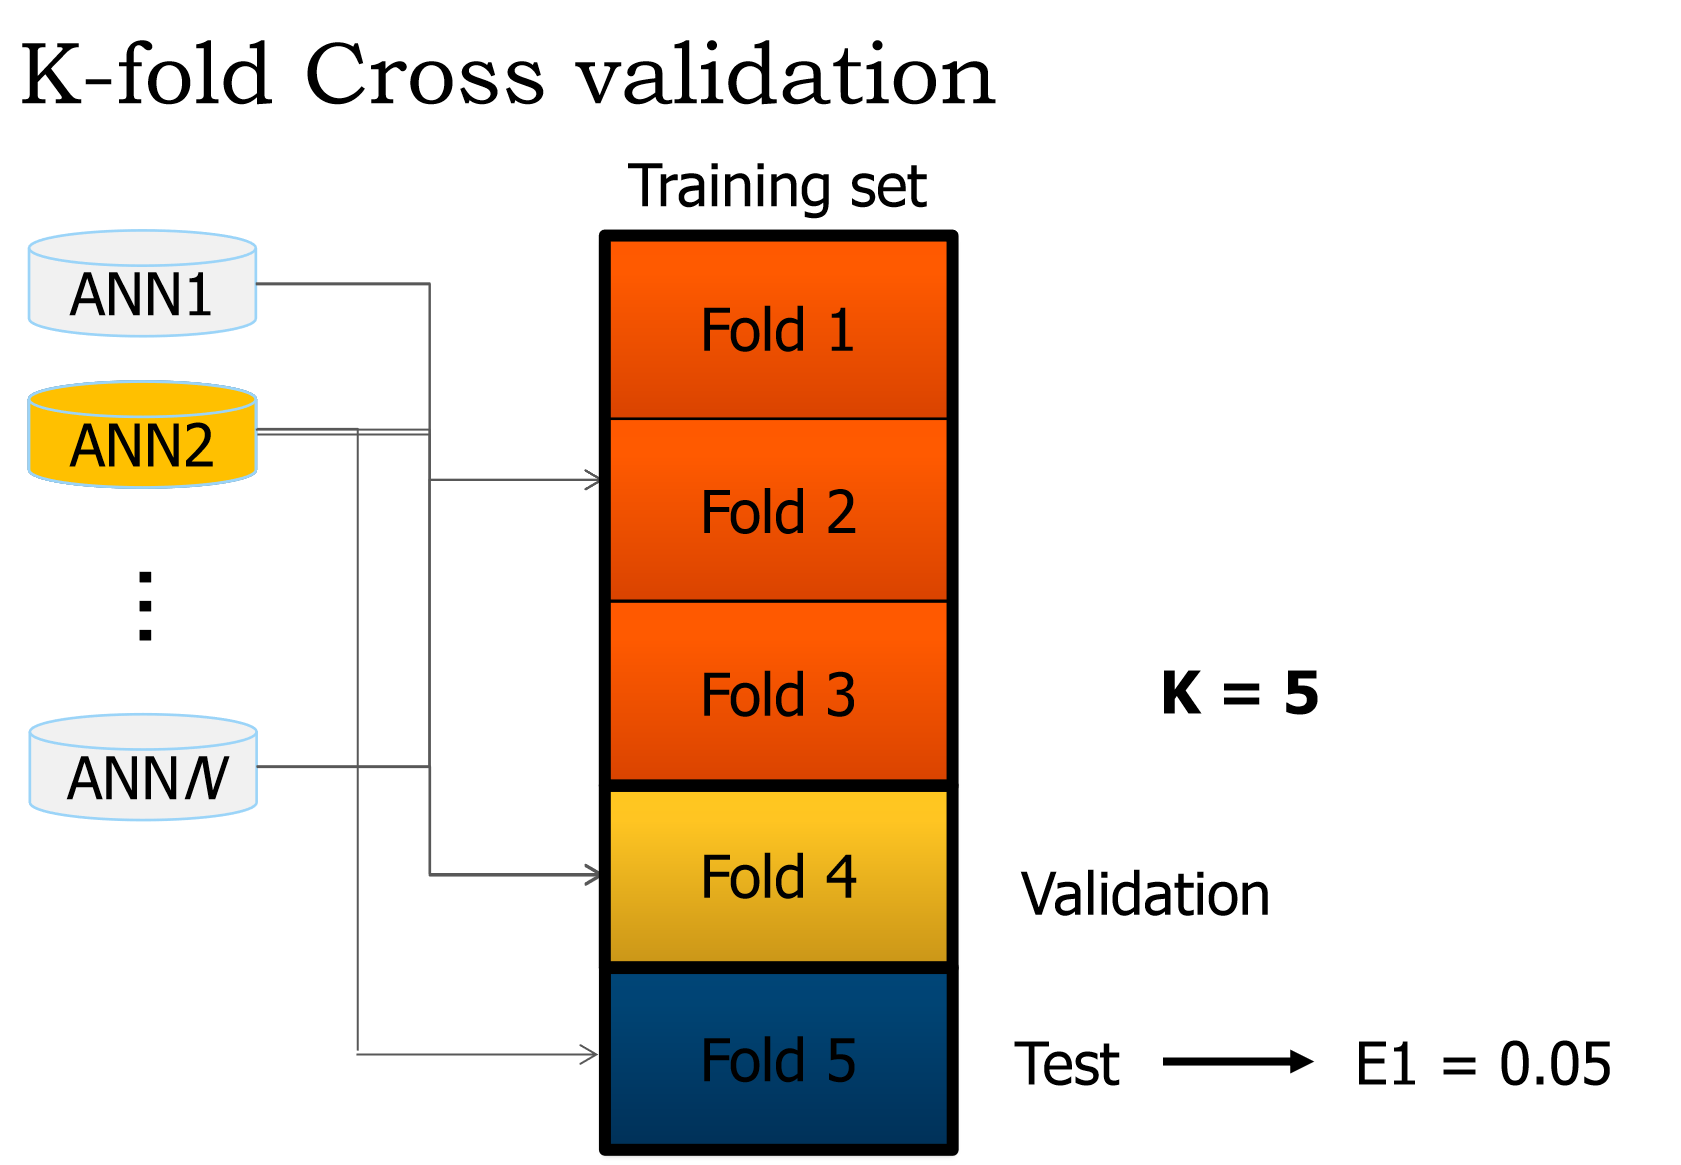
\includegraphics[width=4cm]{figures/1174054/2/kfold.png}
		\centering
		\caption{K-fold Cross Validation}
\end{figure}

\item Decision Tree \\
Decision Tree adalah salah satu model prediksi dengan menggunakan struktur pohon atau strktur yang berhirarki. Konsepnya adalah mengubah data menjadi decesion tree dan beberapa aturan keputusan. Decicion Tree memiliki manfaat yaitu membrekdown porses pengambilan keputusan yang kompleks menjadi lebih simpel sehingga pengambil keputusan akan lebih mengintrpretasikan solusi dari suatu permasalahan.
\begin{figure}[H]
		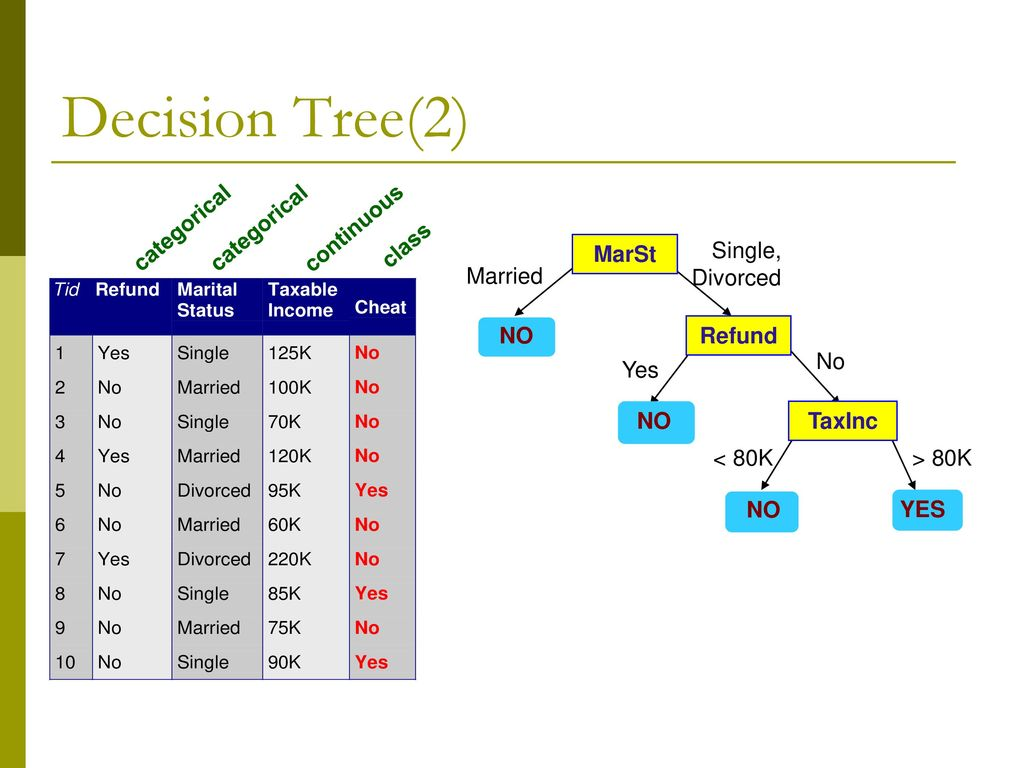
\includegraphics[width=4cm]{figures/1174054/2/decision.jpg}
		\centering
		\caption{Decicion Tree}
\end{figure}

\item Information Gain dan Entropi\\
Information Gain adalah suatu teknik yang didasarkan pada penurunan entropi setelah dataset dibagi pada atribut. Membangun keputusan adalah menemukan atribut yang mengembalikan perolehan informasi tertinggi.
\begin{figure}[H]
		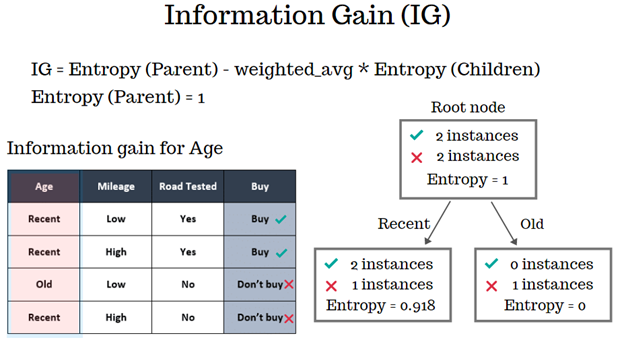
\includegraphics[width=4cm]{figures/1174054/2/information.png}
		\centering
		\caption{Information Gain}
\end{figure}

Entropi adalah suatu ukuran acak dalam informasi yang sedang diproses. Semakin tinggi sutau entropi, semakin sulit menarik kesimpulan dari informasi tersebut. Decision tree dibangun dari atas kebawah dan melibatkan partisi data kedalam himpunan bagian yang berisi instance dengan nilai yang sama. Algoritma ID3 menggunakan entropi untuk menghitung suatu homogenitas sampel. 
\begin{figure}[H]
		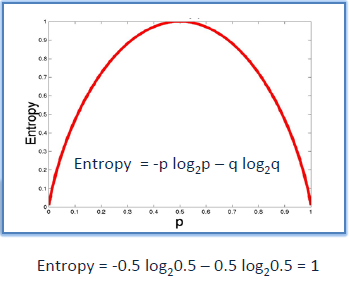
\includegraphics[width=4cm]{figures/1174054/2/entropy.png}
		\centering
		\caption{Entropy}
\end{figure}
\end{enumerate}

\subsection{Praktek}
\begin{enumerate}
\item Nomor 1
\hfill\break
	\lstinputlisting[firstline=10, lastline=14]{src/1174054/2/1174054.py}
Hasilnya :
\begin{figure}[H]
		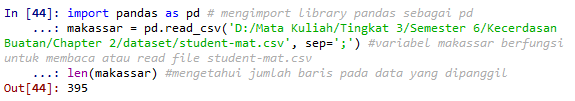
\includegraphics[width=4cm]{figures/1174054/2/1.png}
		\centering
		\caption{Hasil Nomor 1}
\end{figure}

\item Nomor 2
\hfill\break
	\lstinputlisting[firstline=18, lastline=22]{src/1174054/2/1174054.py}
Hasilnya :
\begin{figure}[H]
		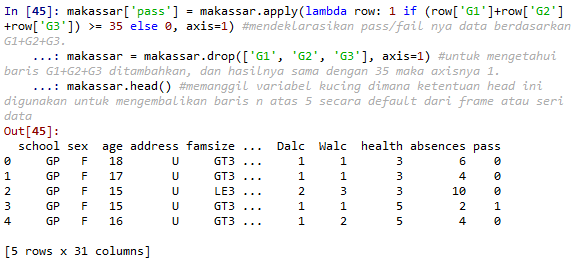
\includegraphics[width=4cm]{figures/1174054/2/2.png}
		\centering
		\caption{Hasil Nomor 2}
\end{figure}

\item Nomor 3
\hfill\break
	\lstinputlisting[firstline=26, lastline=31]{src/1174054/2/1174054.py}
Hasilnya :
\begin{figure}[H]
		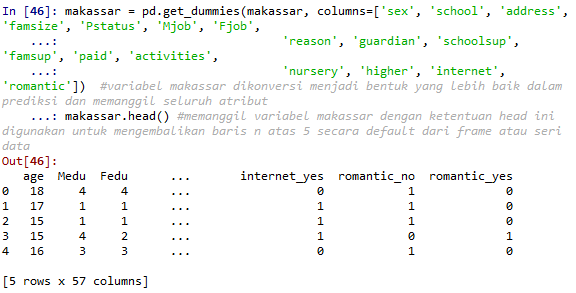
\includegraphics[width=4cm]{figures/1174054/2/3.png}
		\centering
		\caption{Hasil Nomor 3}
\end{figure}

\item Nomor 4
\hfill\break
	\lstinputlisting[firstline=35, lastline=53]{src/1174054/2/1174054.py}
Hasilnya :
\begin{figure}[H]
		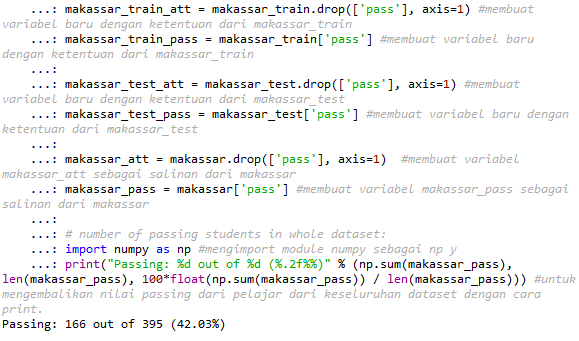
\includegraphics[width=4cm]{figures/1174054/2/4.png}
		\centering
		\caption{Hasil Nomor 4}
\end{figure}

\item Nomor 5
\hfill\break
	\lstinputlisting[firstline=57, lastline=61]{src/1174054/2/1174054.py}
Hasilnya :
\begin{figure}[H]
		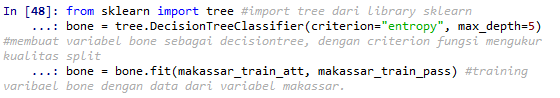
\includegraphics[width=4cm]{figures/1174054/2/5.png}
		\centering
		\caption{Hasil Nomor 5}
\end{figure}

\item Nomor 6
\hfill\break
	\lstinputlisting[firstline=65, lastline=74]{src/1174054/2/1174054.py}
Hasilnya :
\begin{figure}[H]
		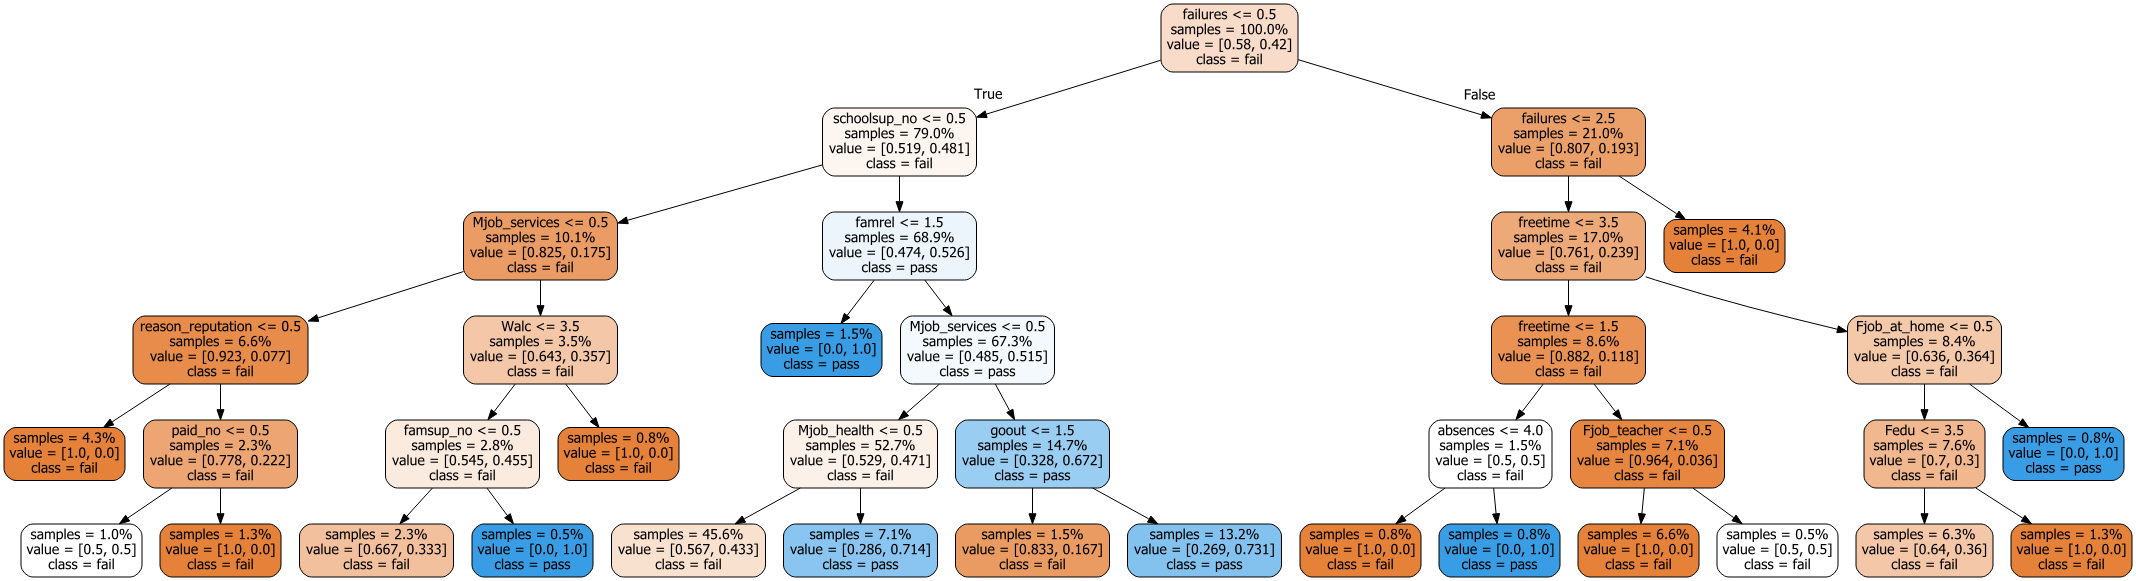
\includegraphics[width=4cm]{figures/1174054/2/6.png}
		\centering
		\caption{Hasil Nomor 6}
\end{figure}

\item Nomor 7
\hfill\break
	\lstinputlisting[firstline=78, lastline=82]{src/1174054/2/1174054.py}
Hasilnya :
\begin{figure}[H]
		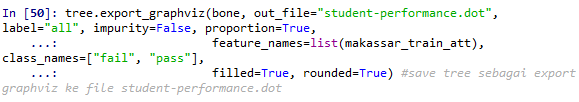
\includegraphics[width=4cm]{figures/1174054/2/7.png}
		\centering
		\caption{Hasil Nomor 7}
\end{figure}

\item Nomor 8
\hfill\break
	\lstinputlisting[firstline=85, lastline=87]{src/1174054/2/1174054.py}
Hasilnya :
\begin{figure}[H]
		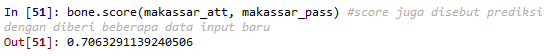
\includegraphics[width=4cm]{figures/1174054/2/8.png}
		\centering
		\caption{Hasil Nomor 8}
\end{figure}

\item Nomor 9
\hfill\break
	\lstinputlisting[firstline=90, lastline=95]{src/1174054/2/1174054.py}
Hasilnya :
\begin{figure}[H]
		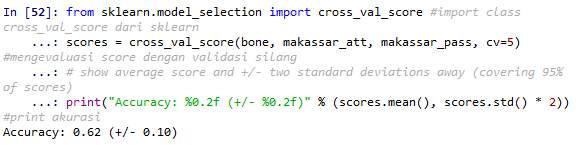
\includegraphics[width=4cm]{figures/1174054/2/9.png}
		\centering
		\caption{Hasil Nomor 9}
\end{figure}

\item Nomor 10
\hfill\break
	\lstinputlisting[firstline=98, lastline=105]{src/1174054/2/1174054.py}
Hasilnya :
\begin{figure}[H]
		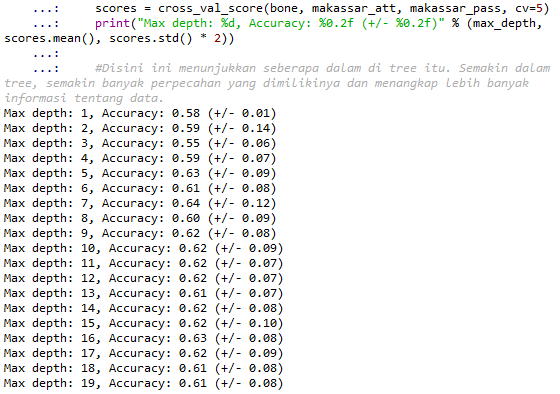
\includegraphics[width=4cm]{figures/1174054/2/10.png}
		\centering
		\caption{Hasil Nomor 10}
\end{figure}

\item Nomor 11
\hfill\break
	\lstinputlisting[firstline=108, lastline=120]{src/1174054/2/1174054.py}
Hasilnya :
\begin{figure}[H]
		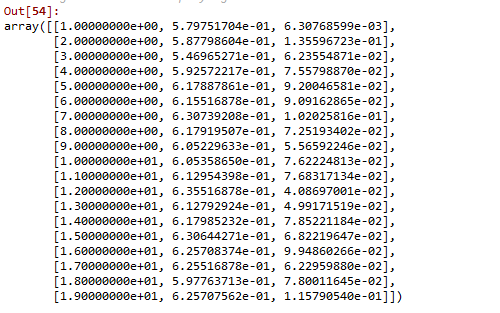
\includegraphics[width=4cm]{figures/1174054/2/11.png}
		\centering
		\caption{Hasil Nomor 11}
\end{figure}

\item Nomor 12
\hfill\break
	\lstinputlisting[firstline=123, lastline=128]{src/1174054/2/1174054.py}
Hasilnya :
\begin{figure}[H]
		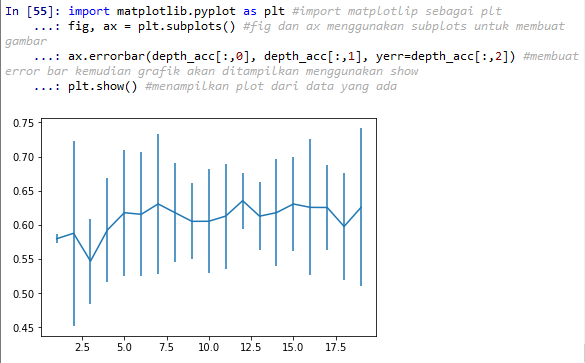
\includegraphics[width=4cm]{figures/1174054/2/12.png}
		\centering
		\caption{Hasil Nomor 12}
\end{figure}
\end{enumerate}
\subsection{Penanganan Error}
\begin{enumerate}
\item ScreenShoot Error
	\begin{figure}[H]
		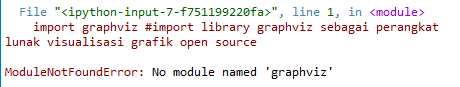
\includegraphics[width=4cm]{figures/1174054/2/error1.png}
		\centering
		\caption{Module Not Found Error}
	\end{figure}
	\begin{figure}[H]
		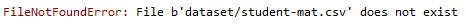
\includegraphics[width=4cm]{figures/1174054/2/error2.png}
		\centering
		\caption{File Not Found Error}
	\end{figure}
	\begin{figure}[H]
		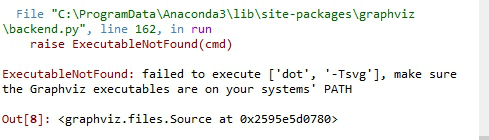
\includegraphics[width=4cm]{figures/1174054/2/error3.png}
		\centering
		\caption{Executable Not Found}
	\end{figure}

	\item Tuliskan Kode Error dan Jenis Error
	\begin{itemize}
		\item Module Not Found Error
		\item File Not Found Error
		\item Executable Not Found
	\end{itemize}
	\item Cara Penanganan Error
	\begin{itemize}
		\item Module Not Found Error
		\hfill\break
		Dengan memperbaiki penulisan atau kesalahan dalam penulisan kode atau melakukan install package atau modul yang belum terinstal
		\item File Not Found Error
		\hfill\break
		Dengan memperbaiki directory file. Sesuaikan sama tempat penyimpanan di laptop
		\item Executable Not Found
		\hfill\break
		Dengan menginstal aplikasi graphviz di windows dan menambahkan directory diatas kode program
	\end{itemize}
\end{enumerate}

\subsection{Bukti Tidak Plagiat}
\begin{figure}[H]
	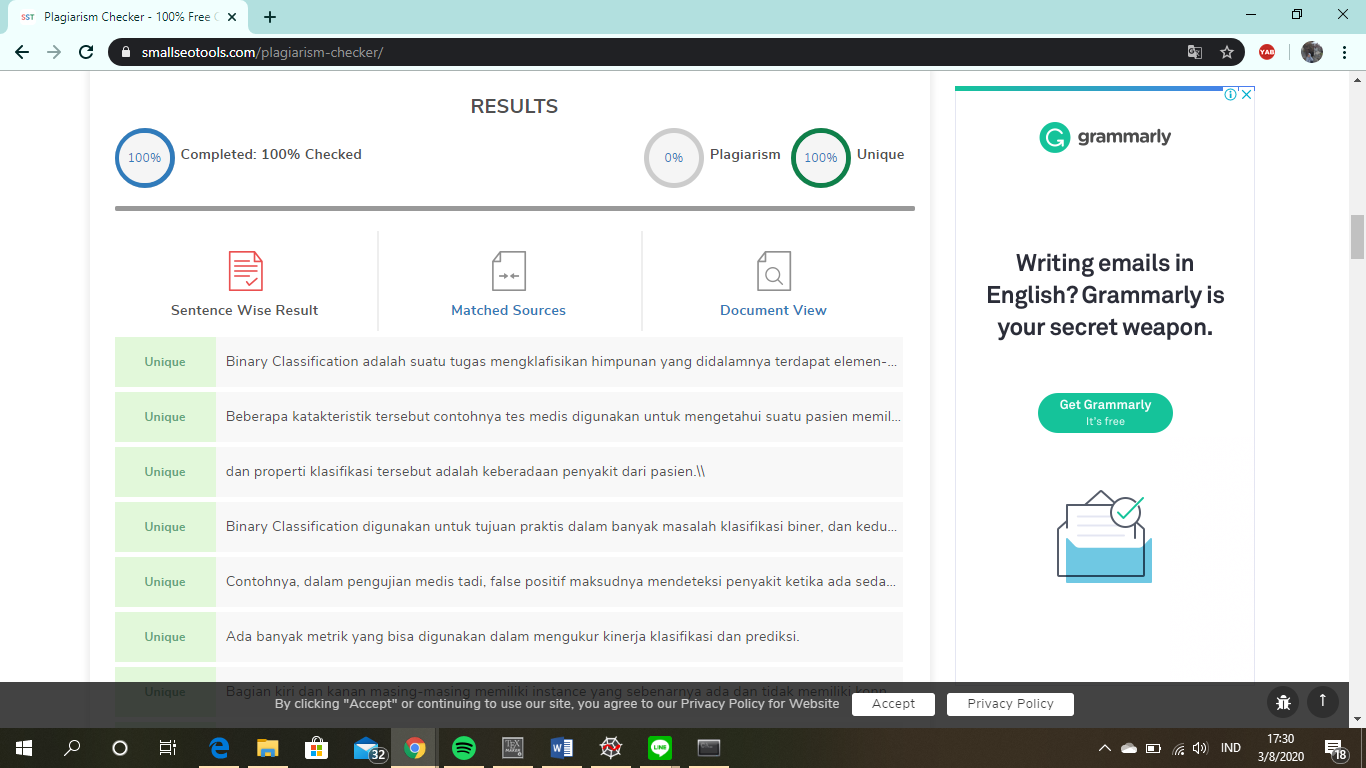
\includegraphics[width=4cm]{figures/1174054/2/plagiarisme.png}
	\centering
	\caption{Bukti Tidak Plagiat}
\end{figure}

\subsection{Link Youtube}
